\section{Risposte alle domande}

\subsection{Domanda 1}
\textit{Misurate i tempi di calcolo dell'algoritmo deterministico di Stoer e Wagner sui grafi del dataset. Mostrate i risultati con un grafico che mostri la variazione dei tempi di calcolo al variare del numero di vertici nel grafo. Confrontate i tempi misurati con la complessità asintotica dell'algoritmo. \\
Nelle istanze più grandi, il tempo di calcolo necessario per completare l'esecuzione potrebbe risultare eccessivo. In questo caso utilizzate un timeout, riportando nei risultati che l'algoritmo non riesce ad ottenere un risultato in tempo utile.}

Abbiamo implementato il codice in Python per l'esecuzione dell'algoritmo di Stoer-Wagner su tutto il dataset fornito. I risultati, che sono stati riportati in modo dettagliato con i relativi pesi anche nella sezione appnedice, sono riportati di seguito.

\begin{figure}[H]
	\centering
	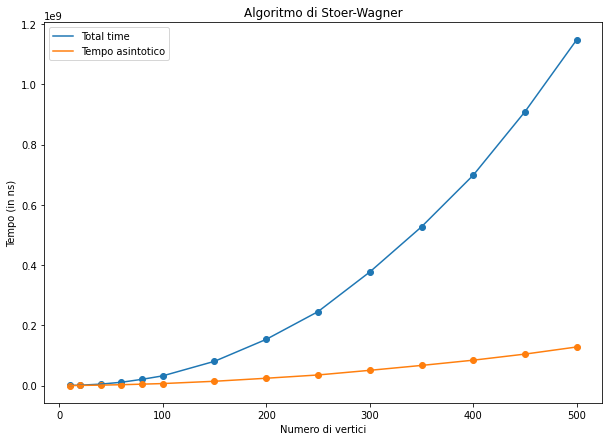
\includegraphics[width=0.85\textwidth]{res/images/single/stoerwagner}
	\caption{Complessità di Stoer-Wagner con \textit{k} esecuzioni ripetute per ogni quartetto di grafi con uguale numero di nodi.}
	\label{fig:stoerwagner}
\end{figure}

Nel grafico appena illustrato (fig. \ref{fig:stoerwagner}) è riportata la complessità computazionale attesa (in giallo) ed effettiva (in blu) per l'algoritmo di Stoer e Wagner con più esecuzioni dell'algoritmo. \\
Come si può evincere dall'immagine, la curva della complessità effettiva rimane al di sopra di quella della complessità teorica. Il motivo di ciò è da ricercare nelle particolarità del linguaggio Python: non ci è stato infatti possibile ridurre le tempistiche di esecuzione per l'algoritmo a causa della necessità di effettuare un \textit{deepcopy} per ogni grafo ad ogni esecuzione, poiché il linguaggio non permette il passaggio di parametri per valore. Sebbene il \textit{deepcopy} sia una procedura che viene eseguita in tempo lineare sulla dimensione dell'oggetto \texttt{graph} (ed ha quindi complessità $O(|V|+|E|)$), essendo l'algoritmo molto veloce questo fattore influisce negativamente sul tempo di esecuzione. \\
Un ulteriore fattore che aumenta la complessità risiede nella rimozione di un nodo dal grafo: essendo l'insieme di vertici un \textit{set}, la rimozione di un elemento da esso ha, nel peggiore dei casi, complessità lineare.

\subsection{Domanda 2}
\textit{Misurate i tempi di calcolo dell'algoritmo di Karger e Stein sui grafi del dataset, usando un numero di ripetizioni che garantisca una probabilità minore o uguale a $1/n$ di sbagliare. Mostrate i risultati con un grafico che mostri la variazione dei tempi di calcolo al variare del numero di vertici nel grafo. Confrontate i tempi misurati con la complessità asintotica dell'algoritmo. \\
Nelle istanze più grandi, il tempo di calcolo necessario a completare tutte le iterazioni potrebbe risultare eccessivo. In questo caso utilizzate un timeout oppure abbassate il numero di ripetizioni per ottenere tempi di esecuzione ragionevoli.}

\subsection{Domanda 3}
\textit{Misurate il discovery time dell'algoritmo di Karger e Stein sui grafi del dataset. Il discovery time è il momento (in secondi) in cui l'algoritmo trova per la prima volta il taglio di costo minimo.  Confrontate il discovery time con il tempo di esecuzione complessivo per ognuno dei grafi nel dataset.}

\begin{figure}[H]
	\centering
	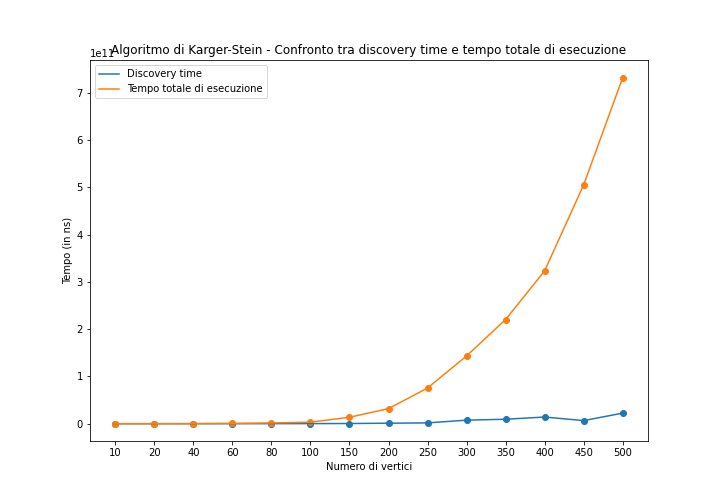
\includegraphics[width=1\textwidth]{res/images/single/karger-stein/discovery-time/karger_stein_confronto_discovery_time_total_time.png}
	\caption{Confronto tra il tempo totale di esecuzione dell'algoritmo e il discovery time per ogni esecuzione.}
	\label{fig:karger_stein_confronto_discovery_time_total_time}
\end{figure}

\begin{figure}[H]
	\centering
	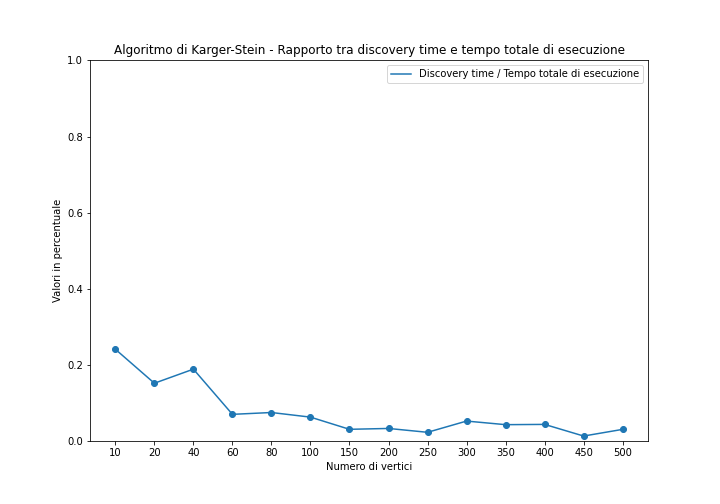
\includegraphics[width=1\textwidth]{res/images/single/karger-stein/discovery-time/karger_stein_rapporto_discovery_time_total_time.png}
	\caption{Rapporto tra il tempo totale di esecuzione dell'algoritmo 
	e il discovery time per ogni esecuzione.}
	\label{fig:karger_stein_rapporto_discovery_time_total_time}
\end{figure}

I valori del grafico \ref{fig:karger_stein_rapporto_discovery_time_total_time} 
esprimono la percentuale di tempo impiegato per trovare per la prima 
volta il min-cut, rispetto al tempo totale di esecuzione dell'algoritmo.

Dai grafici \ref{fig:karger_stein_confronto_discovery_time_total_time} 
e \ref{fig:karger_stein_rapporto_discovery_time_total_time} è possibile 
notare che per le istanze più piccole, il rapporto tra il discovery 
time e il tempo totale di esecuzione è maggiore rispetto allo stesso 
rapporto per le istanze più grandi.

L'esecuzione dell'algoritmo con la threshold a 10 secondi impiega, in media, 
impiega un tempo maggiore per determinare il min-cut. È possibile notare che 
l'esecuzione dell'algoritmo senza threshold impiega un tempo maggiore rispetto 
alle esecuzioni con la threshold. Questo perchè le istanze più grandi richiedono 
un tempo maggiore per poter determinare il min-cut. Tuttavia, l'esecuzione senza 
threshold non ha prodotto errori rispetto al min-cut ottimo. Si illustrino i 
risultati:

Senza threshold: 4.5 secondi;
Threshold di 6 secondi: 2.7 secondi;
Threshold di 10 secondi: 3.1 secondi.

\begin{figure}[H]
	\centering
	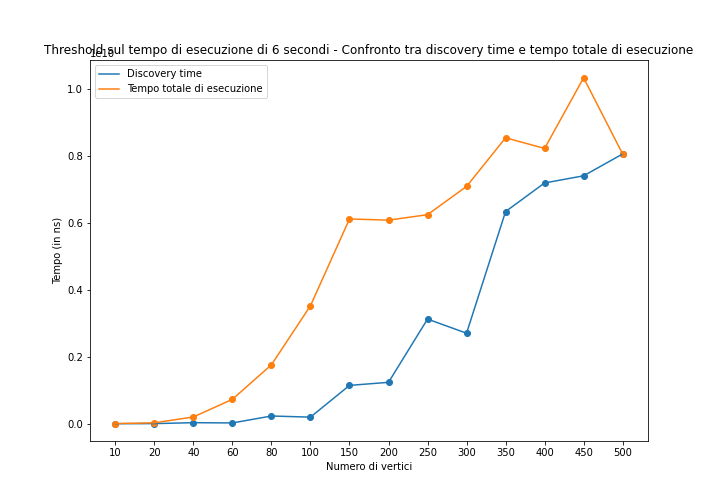
\includegraphics[width=1\textwidth]{res/images/single/karger-stein/discovery-time/threshold6/karger_stein_confronto_discovery_time_total_time_threshold_6s.png}
	\caption{Confronto tra il tempo totale di esecuzione dell'algoritmo e il discovery time per ogni esecuzione.}
	\label{fig:karger_stein_confronto_discovery_time_total_time_threshold_6s}
\end{figure}

\begin{figure}[H]
	\centering
	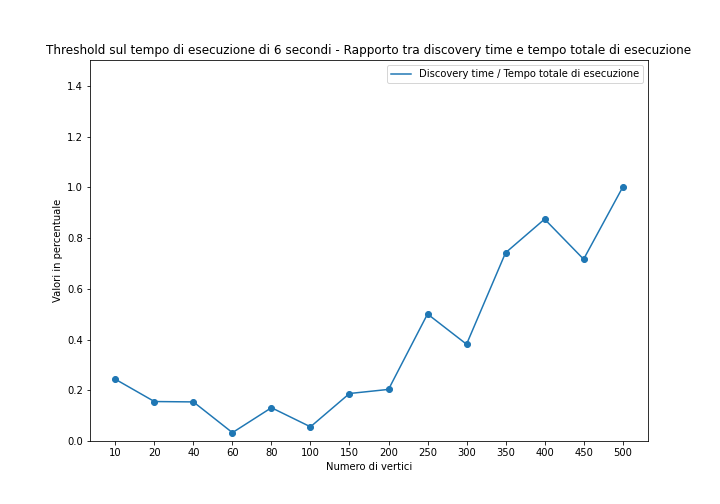
\includegraphics[width=1\textwidth]{res/images/single/karger-stein/discovery-time/threshold6/karger_stein_rapporto_discovery_time_total_time_threshold_6s.png}
	\caption{Rapporto tra il tempo totale di esecuzione dell'algoritmo 
	e il discovery time per ogni esecuzione.}
	\label{fig:karger_stein_rapporto_discovery_time_total_time_threshold_6s}
\end{figure}

\begin{figure}[H]
	\centering
	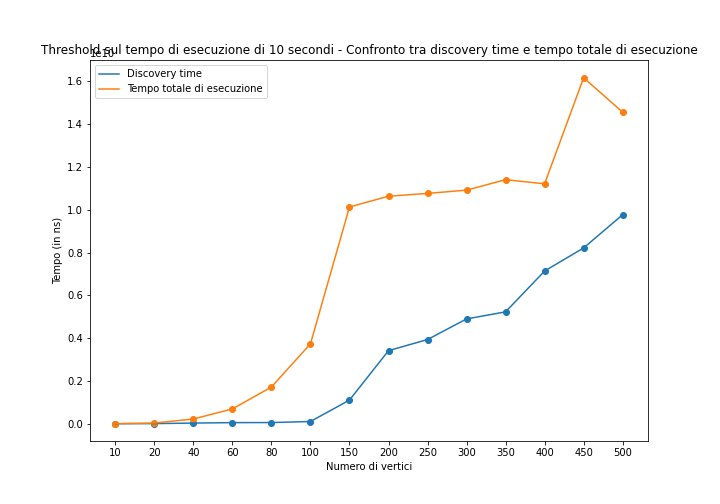
\includegraphics[width=1\textwidth]{res/images/single/karger-stein/discovery-time/threshold10/karger_stein_confronto_discovery_time_total_time_threshold_10s.png}
	\caption{Confronto tra il tempo totale di esecuzione dell'algoritmo e il discovery time per ogni esecuzione.}
	\label{fig:karger_stein_confronto_discovery_time_total_time_threshold_10s}
\end{figure}

\begin{figure}[H]
	\centering
	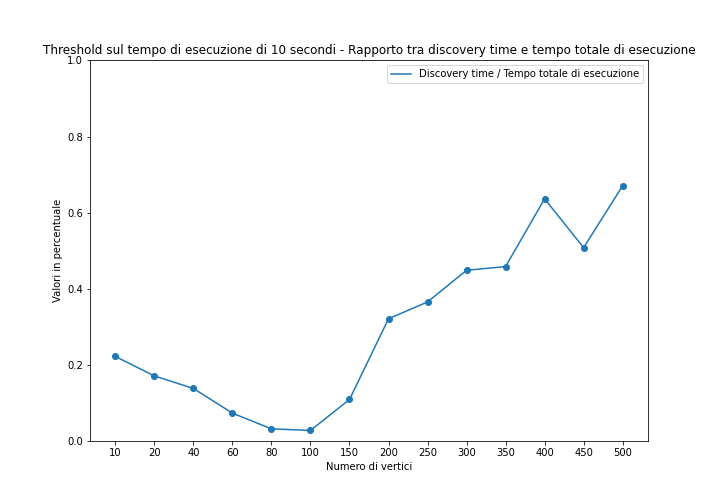
\includegraphics[width=1\textwidth]{res/images/single/karger-stein/discovery-time/threshold10/karger_stein_rapporto_discovery_time_total_time_threshold_10s.png}
	\caption{Rapporto tra il tempo totale di esecuzione dell'algoritmo 
	e il discovery time per ogni esecuzione.}
	\label{fig:karger_stein_rapporto_discovery_time_total_time_threshold_10s}
\end{figure}

\subsection{Domanda 4}
\textit{Per ognuno dei grafi del dataset, riportate il costo del taglio minimo trovato dai due algoritmi. Per l'algoritmo di Karger e Stein, riportate l'errore relativo calcolato come $SoluzioneTrovata-SoluzioneOttima/SoluzioneOttima$, dove $SoluzioneOttima$ è la soluzione trovata dall'algoritmo deterministico, se esiste.}

L'esecuzione dell'algoritmo di Karger-Stein senza la threshold sul 
tempo di esecuzione ha sempre restiuito la soluzione ottima. Invece, 
imponendo una threshold sul tempo esecuzione è possibile notare dal 
grafico \ref{fig:karger_stein_tassi_di_errore} che l'algoritmo 
comincia a restituire delle soluzioni con una maggiore imprecisione 
a mano a mano che la dimensione dell'istanza aumenta.

Nel grafico è possibile notare che aumentando la threshold 
(da 6 secondi a 10 secondi), l'algoritmo produce delle soluzioni più 
precise, ovvero, il tasso di errore diminuisce. In particolare, 
l'algoritmo diventa più preciso a mano a mano che la dimensione delle 
istanze aumenta.

\begin{figure}[H]
	\centering
	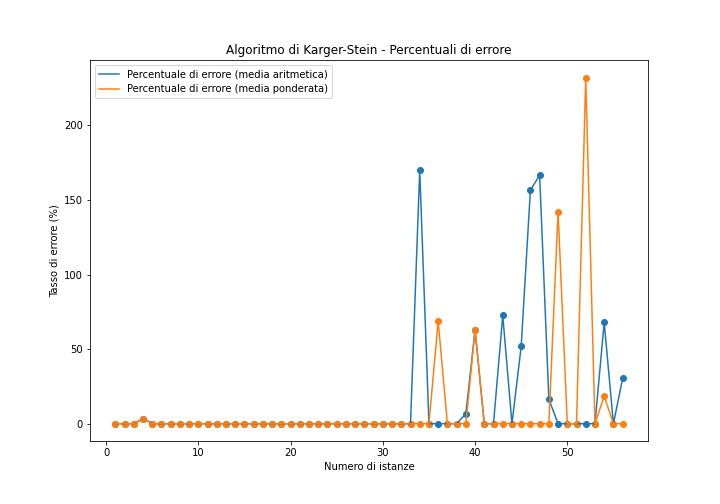
\includegraphics[width=1\textwidth]{res/images/single/karger-stein/tasso-di-errore/karger_stein_tassi_di_errore.png}
	\caption{Variazione del tasso di errore al variare della threshold
	(blu = threshold di 6 secondi, arancione = threshold di 10 secondi).}
	\label{fig:karger_stein_tassi_di_errore}
\end{figure}

\subsection{Domanda 5}
\textit{Commentate i risultati che avete ottenuto: come si comportano gli algoritmi rispetto alle varie istanze? C'è un algoritmo che riesce sempre a fare meglio degli altri? Quale dei due algoritmi che avete implementato è più efficiente? Quale il più preciso nei risultati?}
